%!TEX root = ../../thesis.tex

%=============================================================================


\section{Library}
\label{main:lib}
In this part of this thesis the library of the proposed framework will described, along with its tasks.
As discussed earlier, the library of the proposed framework solves a number of problems, which are either directly needed for synchronization of results or make it considerably easier.
First the reasoning for some major design decision will be laid down.
After this more technical details and explanations will follow.


% audio transmission
\subsubsection{Audio Formats}
\label{main:lib:formats}
One of the central tasks of the library involves transmitting audio from component to component.
This includes some aspects not immediately obvious.
One of those is the audio format each component requires.
An audio format determines the structure of the audio data on a lower level.
Typically, the structure of any audio data can be described by four factors:
\begin{enumerate}
	\item Its \textit{Samplerate}, which determines the resolution of an audio signal is in time domain.
	\item Its \textit{Bitrate}, which determines the resolution of the singular data points within a audio signal.
	\item Its \textit{Endianness}, which determines the order of bytes of the singular data points within a audio signal. Litte-endian encoding puts the least significant bytes first, while big-endian encoding puts the most significant bytes first. 
	\item Its \textit{Channel Count}, which determines the number of distinct audio signals within the signal. When recording audio, the \textit{Channel Count} is generally equivalent to the number of microphones used to record the audio signal.
\end{enumerate}
Working on audio data which is present in a different format then expected will in most cases lead to unusable results, maybe even to critical segmentation faults. 

Under normal circumstances, a component will request audio in the format it requires directly, e.g. via \gls{alsa}.
However, as the library now handles all audio transmission, this is no longer feasible.
With respect to one of the secondary goals of this thesis, to provide a modular framework, every components algorithm can also not be assumed to work with a specific audio format.
This leaves us to either require each component to use a single, pre-determined audio format or resampling and converting audio signals for each component.
By handling resampling and converting of audio signals within the library, components of the resulting framework can theoretically employ any kind of algorithm they desire, without having to handle resampling and converting audio themselves.
Furthermore, by abstracting resampling and converting from the components themselves, the library can be equipped to change audio formats adaptively when new components are introduced or old components vanish from a specific configuration, in a standardized way.

Consequently, the library needs to be able to resample and convert audio between arbitrary audio formats.
We chose the \gls{soxr} library \cite{soxr,soxrbase}, to resample the audio and use a custom implementation to change its \textit{Bitrate}.
The library does not handle different \textit{Channel Counts}.
The reason for this is the absence of a sufficient default behavior.
While creating a two channel audio signal from a single channel is easily done by doubling it, how to convert a two channel signal with non-identical tracks into a three channel signal?
What about the other way round?
Should a two channel signal be interpolated from a three channel signal, or should one of the tracks be discarded?
The answers to these questions differ from case to case.
As such, it seems more wise to separate the channel mechanics into dedicated components and entrust the user with finding the best choice. 
We prepared the library to handle different \textit{Endianness}, but ultimately did not implement such a feature, as different byte order is mostly a historic phenomenon and most modern operating systems, such as Windows, MacOs and most Unix systems, use little-endian encoding.

From the perspective of the library, it can then be divided between an externally used format, which is the format in which the component provides or requests audio data to the library; and an internally used format, which is the format in which the audio is transmitted.
Both of these can be identical, but must not be.
Resampling and converting of audio signals should be minimized, so careful consideration is required when choosing the format with which to transmit audio between components.

\subsubsection{Audio Format choosing}
\label{main:lib:format_chooosing}
It is however equally important where these formats are chosen, as it could be done in two ways:
Either in a distributed manner, where all existing components must communicate with each other and come to a single conclusion.
Alternatively they could be determined in a centralized manner, where a single master program will collect information about each component and then based on this information will make a decision.
This was the chosen course of action, which was motivated as follows:
The main advantage of a distributed approach is that it does not rely on an additional program, as does the centralized approach.
It does so however at a cost. 
Due to the nature of the distributed approach each component taking part must have the same information as each other, that is to say each component must have information about at least each other component.
See for example figure \ref{pic:main:lib:central_vs_dist}.
In this scenario of average complexity one can clearly see the centralized approach to introduce less overhead.
While the communication between \texttt{c\_1} and \texttt{c\_2} is straight forward within the distributed approach, the communication between \texttt{c\_2}, \texttt{c\_3}, \texttt{c\_4} and \texttt{c\_5} becomes quite convoluted.
Additionally, the way in which each format is determined must be deterministic, as each component must come to the same conclusion.
All this results in a not insignificant overhead in both computational load and inter-component communication.

\subsubsection{General Requirements}
However, as there is already always an additional program  employed to synchronize the results, namely the Orchestrator, the benefit of the distributed approach becomes negligible.
We thus chose to implement the centralized approach with the Orchestrator as the master component, which determines each components internally used audio format.
We will go into detail how the Orchestrator chooses these formats in the following section \ref{main:orc}.

\begin{figure}[]
	\centering
	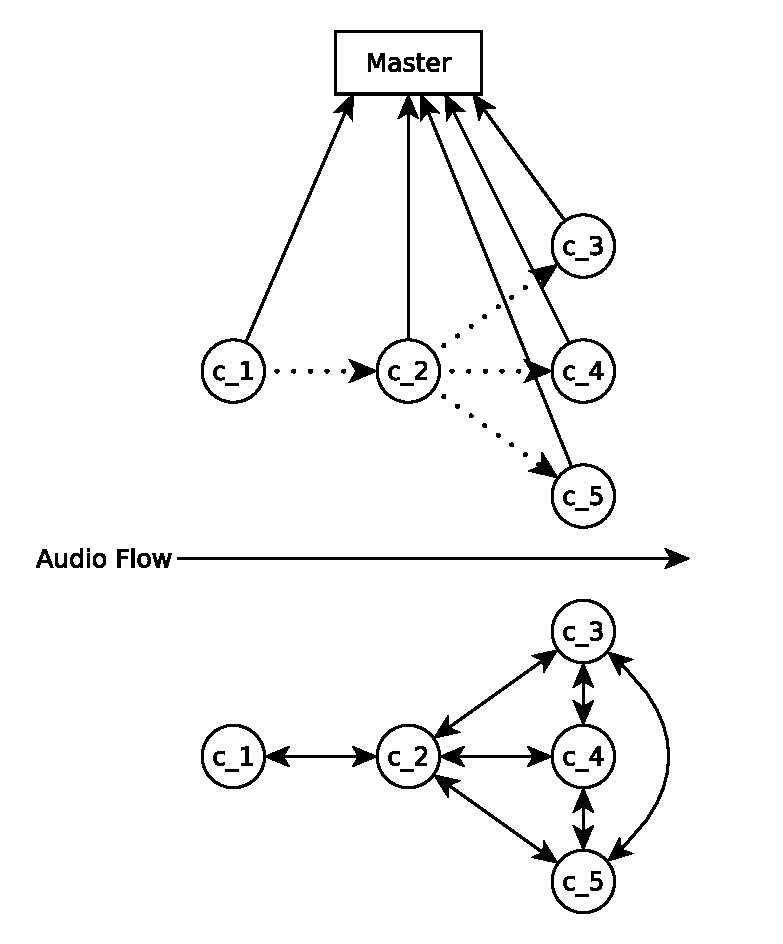
\includegraphics[width=0.66\textwidth]{diagrams/lib_central_vs_dist.pdf}
	\caption{Centralized (above) versus distributed (below) approach of determining audio formats between the components \texttt{c\_1} to \texttt{c\_5}.
		Information sending about each nodes preferred audio topic format are indicated by arrows.
		The direction of audio transmission is indicated by pointed lines above, and from left to right generally speaking.}
	\label{pic:main:lib:central_vs_dist}
\end{figure}

% python bindings
Our library was developed in C++, do to it having access to a number of very widely used and tested libraries for audio processing, such as \gls{sox} as well as its speed.
However, a number of interesting software was developed for Python, see for example libraries on which I based most of the developed components, discussed below in chapter \ref{main:components:start}.
This is what drove us to develop Python bindings for the library, using Boost Python \cite{Abrahams2003BuildingHS}.
It proved fruitful, as most the then developed components actually make use of these bindings rather then the original C++ library.
Developing the library in Python in the first place was considered, but ultimately not chosen because of C++'s superior support with regards to sound libraries, such as \gls{sox} and \gls{soxr}.

\subsubsection{Result Types}
\label{main:lib:message_types}
Another important task of the library is to provide standardized \gls{ros} messages of common results generated from raw audio.
This is realized by a number of \gls{ros} messages, dedicated to speech-, emotion-, gender-, voice-, \gls{ssl}-, and \gls{vad}- information.
These messages can be inspected in figure \ref{table:main:lib:messages}.
They generally consist of a start \& end timestamp, a probability and a string containing their actual result.
Special cases are the \textit{VADInfo} message, which lacks such a string, as it only needs to capture a timeframe, 
the \textit{SpeechInfo} message, which consists of a list of result strings and their respective probabilities, along with an duration, 
and the \textit{SSLInfo} message, which in addition to a duration fields a list of \gls{ssl} outcomes, determined by an vertical as well as horizontal angle and a distinct source ID.
In any case, these must be published by the components to similarly standardized \gls{ros}-topics, consisting of the name of the component and the type of the message.

\begin{figure}[]
	\centering
	\begin{tabular}{| l | l |}
		\hline
		\multicolumn{2}{|c|}{\textbf{Duration}} \\\hline
		start & finish \\\hline
	\end{tabular}\\\vspace{0.3cm}
	
	\begin{tabular}{| l | l | l |}
		\hline
		
		\multicolumn{3}{|c|}{\textbf{GenderInfo}} \\ \hline
		gender* & probability & Duration \\\hline
	\end{tabular}\\\vspace{0.3cm}
	
	\begin{tabular}{| l | l | l |}
		\hline
		
		\multicolumn{3}{|c|}{\textbf{EmotionInfo}} \\ \hline
		emotion* & probability & Duration  \\\hline
	\end{tabular}\\\vspace{0.3cm}
	
	\begin{tabular}{| l | l | l |}
		\hline
		
		\multicolumn{3}{|c|}{\textbf{VoiceIdInfo}} \\ \hline
		voiceId* & probability & Duration  \\\hline
	\end{tabular}\\\vspace{0.3cm}
	
	\begin{tabular}{| l | l |}
		\hline
		
		\multicolumn{2}{|c|}{\textbf{VADInfo}} \\ \hline
		probability & Duration  \\\hline
	\end{tabular}\\\vspace{0.3cm}
	
	\begin{tabular}{| l | l | l |}
		\hline
		
		\multicolumn{3}{|c|}{\textbf{SpeechInfo}} \\ \hline
		\multicolumn{2}{|c|}{hypotheses[]} & Duration  \\\cline{1-2}
		recognizedSpeech* & probability & \\\hline
	\end{tabular}\\\vspace{0.3cm}
	
	\begin{tabular}{| l | l | l | l|}
		\hline
		
		\multicolumn{4}{|c|}{\textbf{SSLInfo}} \\ \hline
		\multicolumn{3}{|c|}{directions[]} & Duration  \\\cline{1-3}
		sourceId* & angleVertical & angleHorizontal & \\\hline
	\end{tabular}\\\vspace{0.3cm}
	
	\begin{tabular}{| l | l | l |}
		\hline
		
		\multicolumn{3}{|c|}{\textbf{EsiafRosMsg}} \\ \hline
		GenderInfo[]	& EmotionInfo[]	& VoiceIdInfo[]	\\\hline
		VADInfo[]	& SpeechInfo[]	& SSLInfo[] \\\hline
	\end{tabular}
	\caption{A list of all available result messages and their composition.
		All entries indicated with a star are of type string and generally used for result transmission.
		All other entries are either of a type shown here (e.g. Duration), or are floats.
		Square brackets indicate this entry to be a list of this type with unspecified length.
		The EsiafRosMsg is a special type reserved for usage by the Orchestrator, as it represents the message of synchronized results.
		}
	\label{table:main:lib:messages}
\end{figure}

%--------------------------------------------------------------------

We will now illustrate the tasks handled by the library by means of typical actions taken by an example component in its life-cycle.
Our example will be that of a typical \gls{vad} component.
As \gls{ros}is used as an underlying middleware, components within the proposed framework must also use \gls{ros} for a number of tasks.
Thus it is necessary for the component to first initialize \gls{ros}.
Following this, the proposed library will need to be initialized, which is done by first creating a handle.
This handle keeps track of all relevant information the proposed library needs.

Our example component may then declare its intention to output or request audio.
In the example, the \gls{vad} component will first declare its intend to output audio and then to require audio.
However, the library does not put a limit as to how many in- \& outputs a component can request, so an identifier is needed.
The same identifier will later internally used to generate the \gls{ros} topics with which the actual audio will be transmitted.
So it also serves to map the audio between components.%todo formulierung
If the \gls{vad} component would use the input topic \texttt{''vad\_input''}, then a microphone component would be needed to output on the same topic, so that the audio could be correctly transmitted.
Also needed to request an audio in- or output is the format in which the audio should arrive or will be given to the library respectively.

When declaring the output of audio, there are no further requirements.
When requesting audio however, the component must present the library with a callback function.
This function will later be invoked when audio was send to the component.

\subsubsection{Raw Audio Transmission}
\label{main:lib:augmented_audio_msg}
Later, when the component is finished initializing the library and is working, % fomulierung
the component will want to actually receive and output audio.
To output audio, it will need to provide the raw audio signal in the format that it chose previously and its timestamps along with the topic on which this audio shall be transmitted.
The library will then convert this raw audio signal and its corresponding timestamps to a \textit{Augmented Audio Message}, as seen in figure \ref{pic:main:lib:augmented_audio}.
The information contained in these messages can be divided into three categories:
\begin{enumerate}
	\item Transmission information
	\item Synchronization information
	\item Meta information
\end{enumerate}
The transmission information consists of the audio signal to be transmitted as well as an message ID.
This ID is generated by the library on the transmitting side and is consecutive.
\gls{ros} as a middleware does not ensure messages to arrive at a node in the same order they were sent.
Thus, by adding an ID to each message, the receiving side of the library can later rearrange the order of arrival, should messages arrive out-of-order.
The library will also resample and convert the raw audio signal it received in the externally used format into the internally used format, if these are not identical.
Depending on the size of audio chunk this part of the message should normally be the largest.
It must be noted however, that because picking the right size of audio chunking is a non-trivial exercise (see chapter \ref{basics:latency}), the library does not give any restrictions on the size of the audio signal to be transmitted.
Even varying the size of the audio chunks between messages is allowed.  

The synchronization information is the part of the message which carries the timestamps corresponding to the audio signal.
It therefore enables components to enhance their results with accurate timestamps which in turn are later synchronized by the Orchestrator.

The last part of the message consists of optional meta information.
These meta information can be \gls{ssl} or \gls{vad} information.
As previously discussed, this information must be published by their respective nodes to the Orchestrator for synchronization purposes.
However, as a special case for \gls{ssl} and \gls{vad} components, they should also enhance the audio information with them.
The reasoning behind this is rather straight forward:
Most beamforming components will need \gls{ssl} information to work correctly.
If these information are not transmitted with the audio signal, the beamformer would need to acquire these information by itself.
After this it would then need to synchronize the \gls{ssl} information with the audio signal.
%This could most probably not be done with the help of the Orchestrator, as a beamformer enhances the audio signal for other components and the Orchestrator would aspire to fuse results by these components with the \gls{ssl} information before outputting them.
We would thus task a component of this thesis proposed framework with the very goal of this thesis.
How absurd this would be.
If these information are however included in the audio signal themselves, they are automatically fused and the beamformer can begin its work outright.
This argument works analogous with \gls{asr} components and the \gls{vad} information.

To enhance an \textit{Augmented Audio Message} with these meta information, a given component must explicitly send them to the library before outputting said \textit{Augmented Audio Message}.
To receive these information, the component must provide the library with a callback function for each.
The receiving component will have all of its callback functions be called in the opposite order.
This process can also be seen in figure \ref{pic:main:lib:ssl_vad_time}.
To come back to the example component:
Our \gls{vad} component would, upon receiving audio, first generate their \gls{vad} information, which it would then publish to the Orchestrator and simultaneously give this information to the library as meta information.
After this it would send the audio signal it received via the library, which would in turn enhance this audio with said \gls{vad} information.
The \textit{Augmented Audio Message} would then arrive in the library of e.g. an \gls{asr} component.
Before anything else, the library would first check the ID of the message.
If it was higher then expected, it would store this message and wait for more messages.
When the expected message arrives, audio signal is resampled and converted from the internally used format to the externally used format.
Then the input callback function of the component would be called with the timestamps and audio signal of the message.
This way the component can use the timestamps directly when publishing results, or just propagate them while outputting audio.
Subsequently the library would call first possible \gls{ssl} and then \gls{vad} meta information callback functions.
Thus it is guaranteed that all audio was processed before information about an ending utterance is given to the component. 
After all callback functions for a given message are called, the library will check for previously but out-of-order received messages and would process them in the same way.



%##########################################

\begin{figure}[]
	\centering
	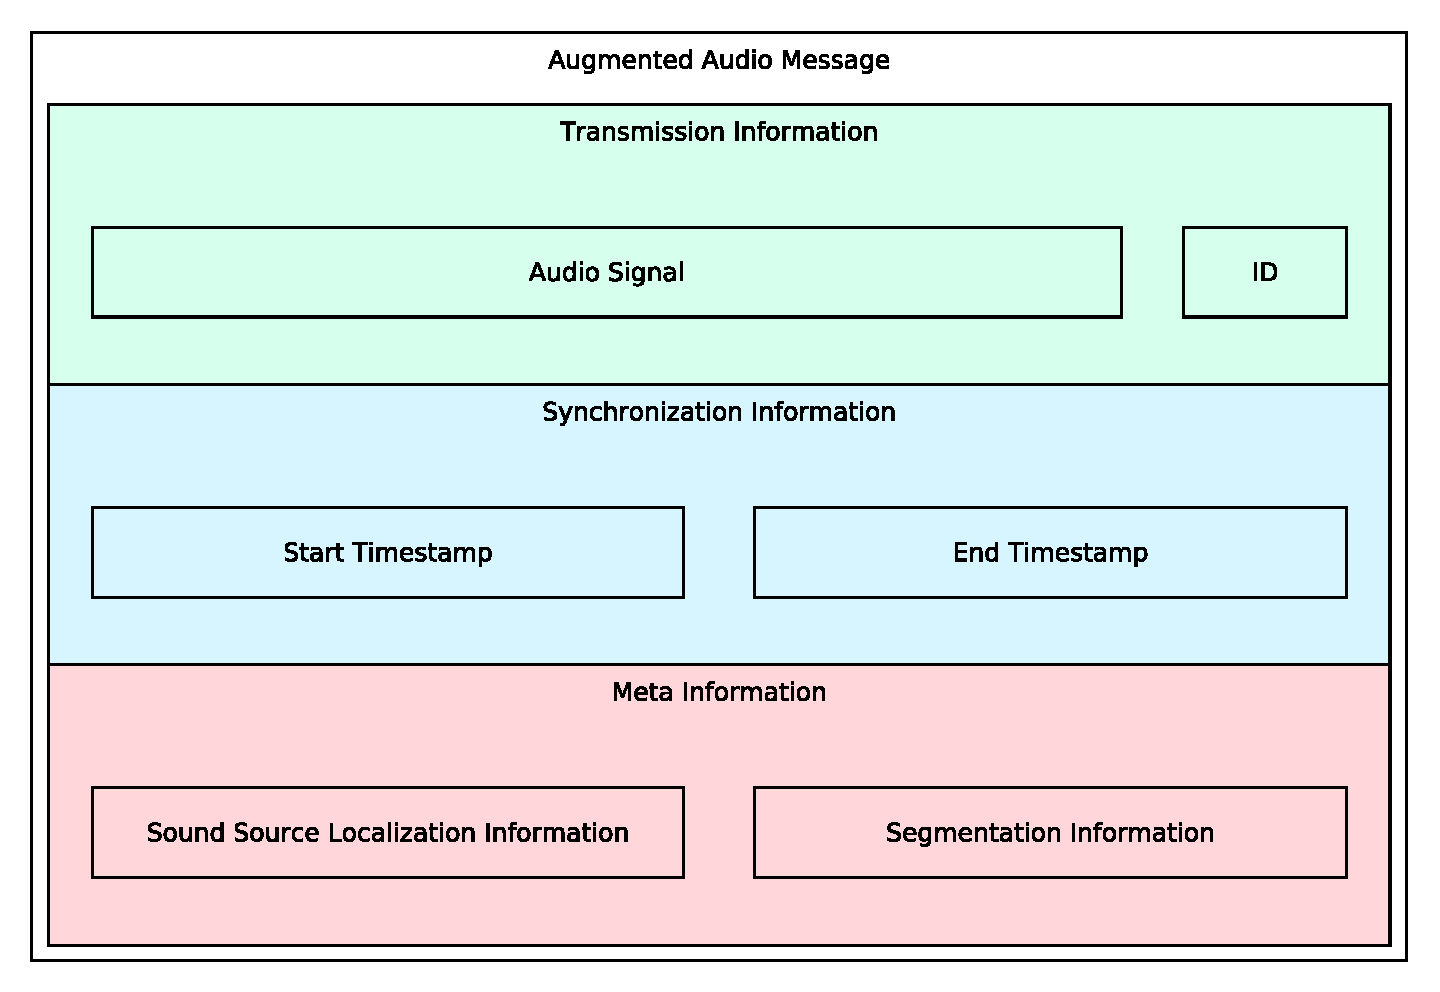
\includegraphics[width=\textwidth]{bilder/rosmsg/augmented_audio.pdf}
	\caption{Composition of Augmented Audio Messages.
		The message can be divided into three parts:
		Transmission information in green, synchronization information in blue, and Meta information in red.}
	\label{pic:main:lib:augmented_audio}
\end{figure}

\begin{figure}[]
	\centering
	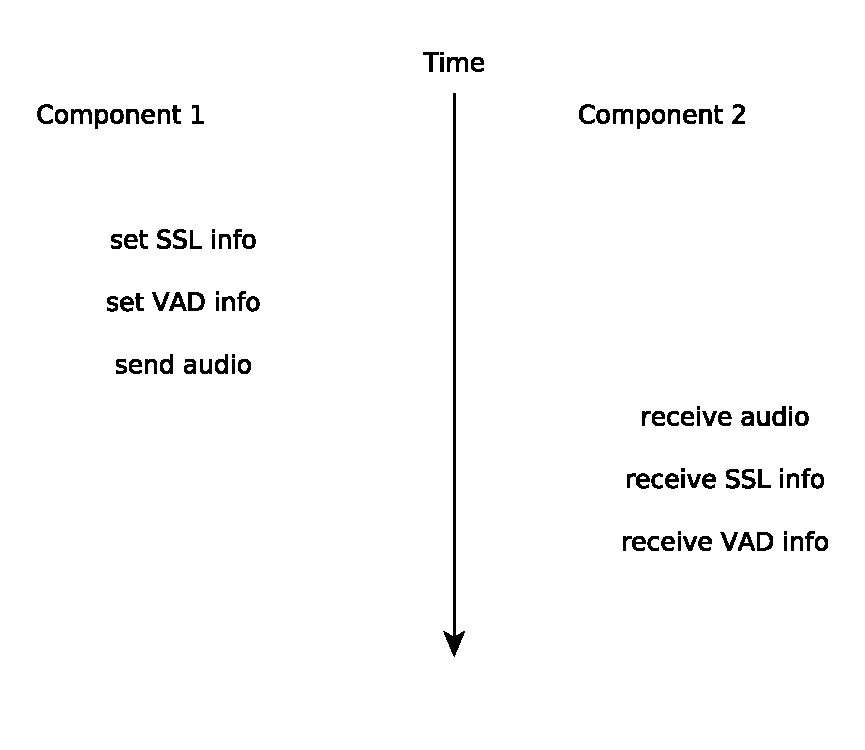
\includegraphics[width=\textwidth]{diagrams/lib_ssl_vad_time.pdf}
	\caption{Timeline of two components sending and receiving \textit{Augmented Audio Messages}.
		One can see the meta information of \gls{ssl} and \gls{vad} to be set before sending the corresponding audio, but being received after it.}
	\label{pic:main:lib:ssl_vad_time}
\end{figure}

\subsubsection{Coordination between Library and Orchestrator}
After the declarations of audio in- \& and outputs are done, the component will signal the library to start.
Up until this point, no actual communication between the component and the Orchestrator has happened.
Now however, the library will prepare all information necessary for the Orchestrator to register the component.
Needed is the name of the component, so the Orchestrator can differentiate components from one another, as well the designation of the node, which corresponds to the task the component will perform.
We will go more into detail regarding this designation in the Orchestrator's chapter \ref{main:orc}, as it serves to easy synchronization of results.

Additionally needed are information about the in- \& output topics of audio that were previously declared.
The information about meta-information are not needed for the registration process, as they are handled internally by the library itself.
Registering the component is then done via a dedicated \gls{ros}-service, which has the library send these information.
Using a \gls{ros}-service in this instance instead of a simple \gls{ros}-message has the advantage, that it can be ensured that the Orchestrator is started and ready, which may not necessarily be the case when starting the Orchestrator and components of the framework in rapid succession.

After this registration has finished, the components work may actually begin.
When the component has finished its work it may signal this to the library, or simply exit.
If the library was thusly informed, it will shut down all audio transmission.
As components cannot be expected to exit in a regulated manner in all cases, the Orchestrator must be able to handle suddenly disappearing components.
Thus there is no dedicated way to de-register a component within the library, and instead the Orchestrator handles all component shut downs.
We will focus on the Orchestrator's approach for this in the following chapter \ref{main:orc}.

